% REMEMBER: You must not plagiarise anything in your report. Be extremely careful.
\documentclass{l4proj}

    
%==============================================================================
% Put any additional packages here
% You can add any packages you want, as long as it does not alter
% the overall format (e.g. don't change the margins or the reference style).
%
\usepackage{pdfpages} % if you want to include a PDF for an ethics checklist, for example
%
%

\begin{document}

%==============================================================================
%% METADATA
\title{Characterising the IETF Through RFC Publication Trends}
\author{Molly Robertson}
\date{October 14, 2026}

\maketitle

\begin{highlight}
\textbf{Research plan:} Compare RFC publication trends across topics and publication statuses, and examine whether references to earlier RFCs relate to changes in document length, status, or team size. Assess whether geographic patterns reflect changes in identifiable author affiliations or gaps in metadata. To address the third research question, compare the distribution of RFCs across indexed topics and working groups over time to assess whether publication has become more concentrated. Check the findings against source documents and note limitations in the available metadata.
\end{highlight}

%==============================================================================
%% ABSTRACT
\begin{abstract}
    Request for Comments (RFCs) are technical documents that the Internet Engineering Task Force (IETF) publishes, documenting fundamental internet protocols, technologies, and standards \cite{IETFProcessRFCs}. As Internet technologies evolve, understanding RFCs and how they have changed over time is vital. Previous studies have examined RFC publication, authorship, deployment, and IETF mailing list activity \citep{McQuistin2021,Khare2022}. However, their analyses only cover data until 2020.

    This project revisits these studies using an updated RFC index snapshot. It measures changes in publication volume, document length, and listed authorship for IETF-stream RFCs published between 1990 and 2026. The results show substantially higher publication activity than at the start of the period, a general reduction in typical RFC length, and an increase in the number of listed authors. The final year's values are treated as provisional because the snapshot may not contain the complete publication year.
\end{abstract}

%==============================================================================
%% ACKNOWLEDGEMENTS
\chapter*{Acknowledgements}
% Enter any acknowledgements here. This is optional; you may leave this blank if you wish,
% or remove the entire chapter
%
% We give thanks to the Gods of LaTeX, who in their eternal graciousness, 
% have granted that this document may compile without errors or overfull hboxes.
%

%==============================================================================

% EDUCATION REUSE CONSENT FORM
% If you consent to your project being shown to future students for educational purposes
% then insert your name and the date below to  sign the education use form that appears in the front of the document. 
% You must explicitly give consent if you wish to do so.
% If you sign, your project may be included in the Hall of Fame if it scores particularly highly.
%
% Please note that you are under no obligation to sign 
% this declaration, but doing so would help future students.
%
%\def\consentname {My Name} % your full name
%\def\consentdate {20 March 2018} % the date you agree
%
\educationalconsent


%==============================================================================
\tableofcontents

%==============================================================================
%% Notes on formatting
%==============================================================================
% The first page, abstract and table of contents are numbered using Roman numerals and are not
% included in the page count. 
%
% From now on pages are numbered
% using Arabic numerals. Therefore, immediately after the first call to \chapter we need the call
% \pagenumbering{arabic} and this should be called once only in the document. 
%
%
% The first Chapter should then be on page 1. 

% PAGE LIMITS
% You are allowed 40 pages for a 40 credit project and 30 pages for a 
% 20 credit report. 
% This includes everything numbered in Arabic numerals (excluding front matter) up
% to but *excluding the appendices and bibliography*.
%
% FORMATTING
% You must not alter text size (it is currently 10pt) or alter margins or spacing.
% Do not alter the bibliography style. 
%
%==================================================================================================================================
%
% IMPORTANT
% The chapter headings and structure here are **suggestions**. You don't have to follow this model if
% it doesn't fit your project. Every project should have an introduction and conclusion,
% however.  If in doubt, your supervisor can give you specific guidance; their view takes precedence over
% the structure suggested here.
%
%==================================================================================================================================
\chapter{Introduction}

% reset page numbering. Don't remove this!
\pagenumbering{arabic} 

% You can use \todo{} to mark text that needs to be fixed. Anything inside will appear as highlighted 
% text in the final copy, and you will also get warnings when you compile (so you don't
% forget to take them out!)
The IETF has developed many of the protocols and technical standards we see in the Internet today. This work is published in RFCs that document this as well as keeping a record of how Internet technologies have evolved. Changes in the number of RFCs published per year, their length, or the number of authors listed can reflect changes in the volume and organisation of this work. The countries recorded for each RFC can also be used to examine the composition of the community and investigate if there may be a link between that and some other interesting statistics. However, this needs to be carefully tracked, the country may not be relevant in some RFCs, and careful work needs to be done to define the concept.

This project builds on previous work by analysing RFC publication and authorship trends using more up-to-date data. Rather than only describing how these trends have changed, it asks what may help explain them, including changes in RFC topics and status, references to earlier RFCs, and the organisations associated with authors. It also examines whether apparent changes in geographic representation reflect author affiliations or differences in metadata coverage.

The project addresses the following research questions:

\begin{enumerate}
    \item To what extent are long-term changes in RFC publication volume, document length, and listed author-team size associated with changes in topic and publication-status mix, and with references to earlier RFCs?
    \item What accounts for changes in the recorded geographic representation of RFC authors: changes in identifiable author affiliations, differences in metadata coverage, or both?
    \item \begin{highlight}
    Has RFC work become more concentrated in particular topics or working groups over time?
    \end{highlight}
\end{enumerate}

\begin{highlight}
To answer the third question, the analysis will compare how RFCs are distributed across topics and working groups in different periods. It will use topic and working-group information recorded in the RFC index, looking at whether a smaller set accounts for a larger share of RFCs over time. Since keyword metadata is incomplete and may change in coverage, the results will be interpreted as evidence about the indexed records rather than a complete measure of RFC topics.
\end{highlight}

Abbreviation use and references to other RFCs provide evidence for examining topic mix and reliance on earlier documents. The analysis will measure mentions of abbreviations in the RFC Editor's list. These are potential explanatory factors, not direct measures of influence or causation.

%==================================================================================================================================
\chapter{Background}
McQuistin et al. examine RFC publication, authorship, geographic representation, and email activity, and model real-world RFC deployment using a labelled sample from a corpus of 8,711 RFCs published through 2020 \citep{McQuistin2021}. Their data finds many statistics including time to publish an RFC in days through the years, RFCs updated in each year, authorship by country and company, and email activity. They report changes like the fact that RFCs that build on existing work and have clear requirements are more likely to be deployed and author demographics and affiliation diversity show no statistically significant impact on deployment. Their deployment model is based on a much smaller labelled sample; 251 RFCs had deployment labels and the expanded feature analysis was limited to 155 RFCs for which the additional data was available. This limits how broadly those model findings can be generalised.

These studies provide useful insights however they only go up to 2020 and rely on a relatively small sample. This motivates revisiting these trends and examining how they have changed over the years.

%==================================================================================================================================
\chapter{Analysis/Requirements}
Previous studies use different data sources and definitions, so the first requirement was to define a scope that could be reproduced from public metadata. The analysis therefore uses the RFC index as its source and includes only RFCs in the IETF stream. This excludes IRTF, IAB, independent, and experimental streams from the main comparison rather than combining documents with different publication processes. The available snapshot covers 1990--2026.

The project requirements were:
\begin{enumerate}
    \item calculate the annual number of IETF-stream RFCs;
    \item measure document length using the page count recorded in the index;
    \item measure authorship using the number of authors listed for each RFC;
    \item report the mean and interquartile range so that the average and the spread of typical RFCs can be compared;
    \item produce a reproducible summary table and visualisation from the source metadata.
\end{enumerate}

%==================================================================================================================================
\chapter{Design}
Each RFC is represented by its publication year, stream, page count, and number of listed authors. Records are first filtered to the IETF stream. For each year, the analysis aggregates the number of RFCs and calculates the mean, first quartile (Q1), and third quartile (Q3) of page count and author count. The Q1--Q3 band contains the middle half of the RFCs for that year; the mean is shown separately as the arithmetic average. Quartiles are estimated using linear interpolation, so a quartile may be fractional even when the underlying measure is an integer. The total number of author slots is also retained in the summary table.

\begin{highlight}
The analysis will compare changes across years and examine whether they coincide with changes in topic, publication status, RFC references, author affiliations, and the concentration of RFCs across topics and working groups. This can identify patterns that may help explain the trends, but cannot establish that one variable caused another to change. The mean is sensitive to unusually long documents or large author lists, while the interquartile range shows the spread of the central half of the observations. The output consists of a yearly CSV summary and a three-panel figure showing publication count, page count, and authorship.
\end{highlight}

%==================================================================================================================================
\chapter{Implementation}
The analysis was carried out using a Python data-processing script. It reads the RFC index, selects RFCs in the IETF stream, and groups the records by publication year. For each year, it calculates the number of RFCs and the mean and interquartile range of page counts and listed authors. These summaries are used to produce the tables and figure presented in the findings.

An additional analysis combines the RFC index with the RFC Editor's errata feed \citep{RFCEditorErrata} to summarise errata, keyword metadata, and working-group labels by RFC and publication year.

%==============================================================================
\chapter{Findings}
\section{Publication volume}
The annual number of IETF-stream RFCs increased from 12 in 1990 to a peak of 434 in 2006. Publication volume then fluctuated at lower levels rather than increasing every year.

\section{Length and authorship}
Figure \ref{fig:rfc-trends} summarises the three measures. Comparing 1990 with the last complete year in this snapshot (2025), mean RFC length fell from 53.0 to 26.4 pages. The Q1--Q3 range also shifted down, from 21--55.75 pages to 12--30.75 pages. Over the same period, mean listed authors per RFC rose from 2.17 to 3.18, and the Q1--Q3 range shifted from 1--2.5 authors to 2--5 authors. These measures indicate a broad shift toward shorter RFCs and larger listed author teams. The 2026 values are shown in the figure but are provisional because the snapshot may not include a complete publication year.

\subsection{Unusually long and highly authored RFCs in 1990}
Two RFCs stand out as much longer than the others published in 1990. RFC 1147, \emph{FYI on a Network Management Tool Catalog}, is a 177-page guide to tools for monitoring and debugging TCP/IP networks \citep{RFC1147}. RFC 1190, \emph{Experimental Internet Stream Protocol: Version 2 (ST-II)}, is a 148-page specification for an experimental protocol that aimed to provide guaranteed service for network streams \citep{RFC1190}. ST-II was assigned IP protocol number 5, which is sometimes associated with the informal name ``IPv5''. Its detailed specification helps explain its length. Both RFCs are included in the results and raise the 1990 mean to 53 pages; without them it would be 31.1 pages, following the trend expected.

Two RFCs also stand out for their number of listed authors. RFC 1164, on applying BGP to routing between autonomous systems, lists five authors \citep{RFC1164}. RFC 1175, a bibliography of resources for people learning about internetworking, lists six \citep{RFC1175}. Both are included in the results and raise the 1990 mean to 2.17 authors per RFC; without them it would be 1.5. Current RFC style guidance generally limits the first-page list to five authors or editors; requests to list more are considered by the stream-approving body \citep{RFC7322}. RFC 1175 predates this guidance, so its six listed authors should be understood in its historical context. These examples help explain the 1990 averages, but do not by themselves explain the longer-term trends.

\begin{figure}[htb]
    \centering
    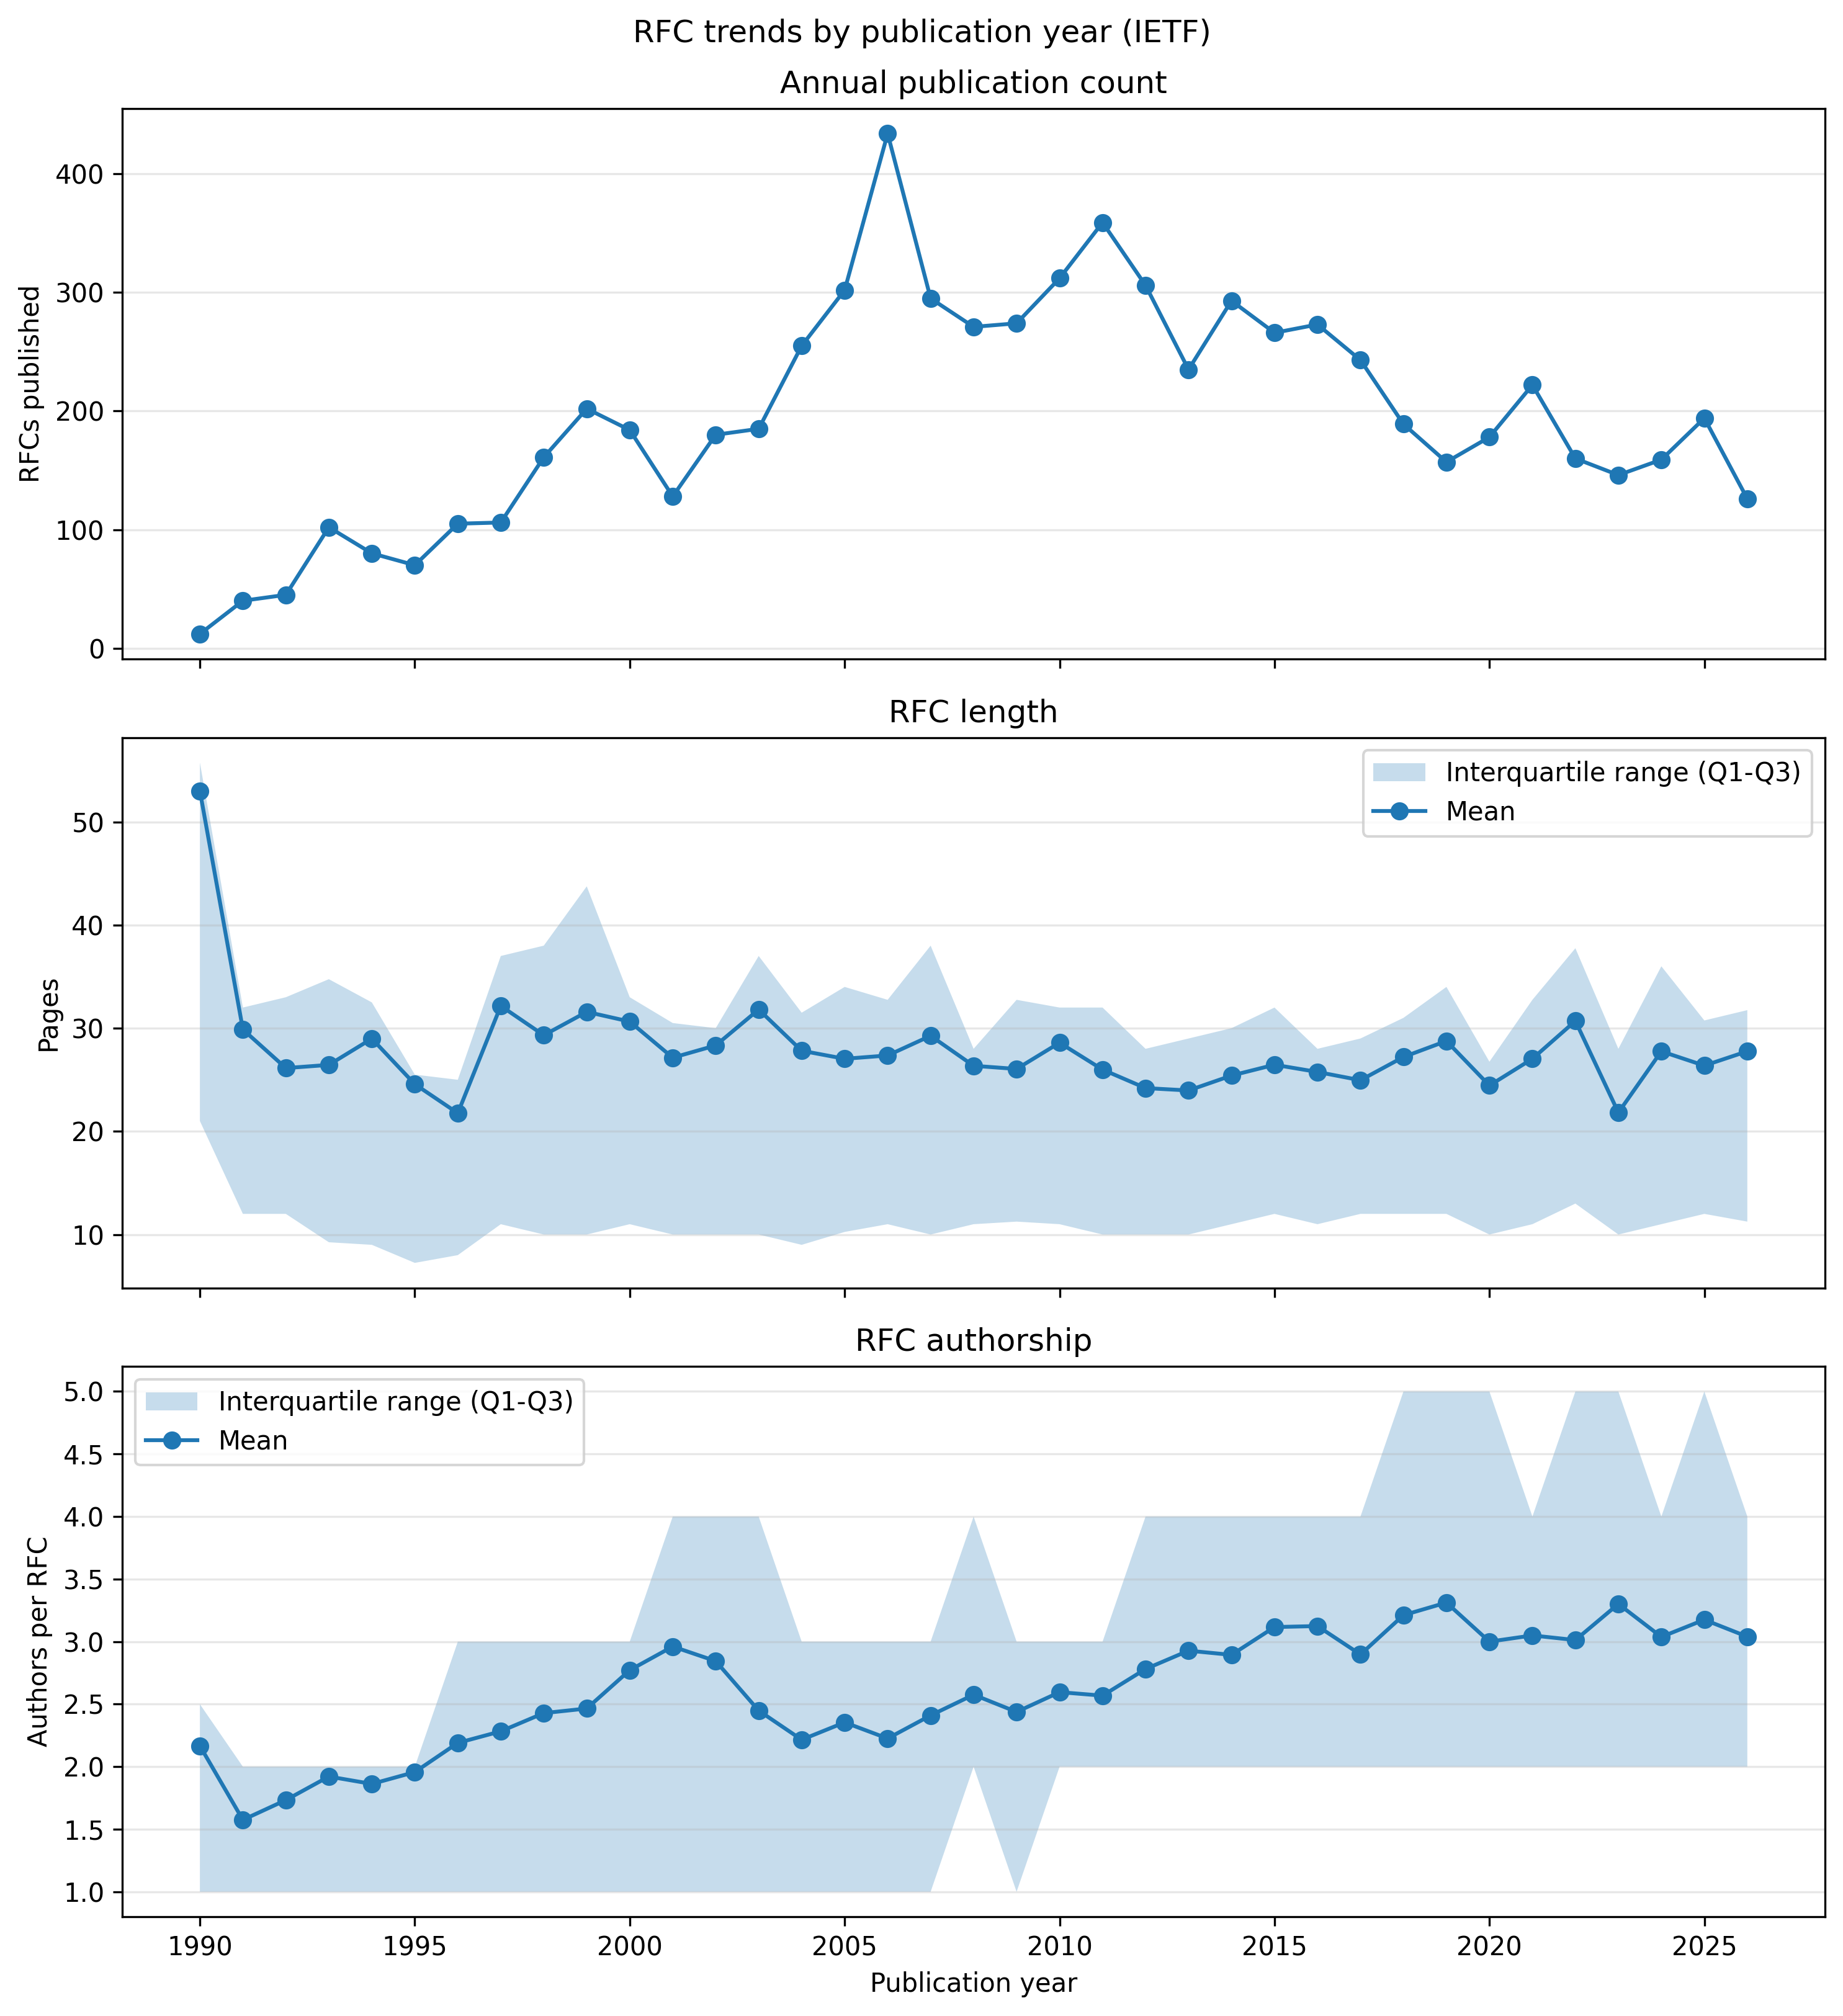
\includegraphics[width=\textwidth]{images/rfc_trends.png}
    \caption{Annual IETF-stream RFC publication count, page count, and listed authorship from 1990 to 2026. For page count and author count, the solid line shows the annual mean and the shaded band shows Q1--Q3 (the interquartile range). The final year's observations may be incomplete.}
    \label{fig:rfc-trends}
\end{figure}

\section{Exploratory indicators of engagement}
Of the 7,249 IETF-stream RFCs in the index, 2,241 (30.9\%) have at least one entry in the RFC Editor's errata feed. Errata are reports of possible corrections, not general comments or a direct measure of how much an RFC is valued. Older RFCs have had more time to accumulate reports, so lifetime totals are not directly comparable.

Comparing RFCs with a complete five-year reporting period, 28.6\% of RFCs published in 2001--2009 and 25.2\% published in 2010--2019 had at least one erratum in that period. This does not suggest a simple increase in reported corrections over time, though reporting practices and the types of RFCs published may differ between periods. Longer RFCs were somewhat more likely to have errata, while the number of listed authors showed little relationship to errata. These patterns do not establish that length causes errors or that team size affects quality.

The working-group labels also suggest that RFCs have been associated with a wider range of groups over time: an average of about 36 distinct group labels appeared each year in the 1990s, compared with about 82 in the 2010s. This points to a broader spread of RFCs across the labels in the index, but does not show how many people participated or how specialised each group was. Indexed keywords vary by decade, with ``protocol'' and ``management'' common in the 1990s, ``SIP'' and ``IPv6'' in the 2010s, and ``security'', ``DNS'', and ``automation'' in 2020--2026. Keyword coverage is incomplete and varies between periods, so these examples should be treated as an indication of topics, not a complete account of how RFC subject matter changed.

% \begin{highlight}
% As a rough check for acronym use, the analysis counted distinct uppercase tokens in each RFC title and abstract. The average rose from 2.56 tokens per RFC in the 1990s to 3.18 in the 2000s, then fell slightly to 3.13 in the 2010s and 3.05 in 2020--2026. This suggests a modest increase from the 1990s, but the measure cannot tell acronyms from other uppercase terms and does not count their use in the full RFC text. It also does not check the RFC Editor's abbreviations list, so it should be read as an exploratory indicator rather than a count of approved abbreviations. \break

% The index records ``updates'' and ``obsoletes'' relationships, but these are not general citation counts. Citation counts are not estimated in the current results because the analysis does not yet include extracted references from RFC text. Taken together, these indicators describe recorded corrections and metadata patterns; they cannot establish whether an RFC was more cared about, adopted, or successful.
% \end{highlight}

\section{Interpretation and limitations}
The simultaneous increase in listed authors and decrease in page count is notable, but the time series cannot establish that one caused the other. One possible interpretation is that technical work has become more specialised and collaborative, with focused documents produced by larger groups; this remains a hypothesis, since this analysis does not measure document topics, team roles, or the relationship between author count and length within each year. Another possible influence is a change in the mix of RFCs: the series contains documents with different purposes and statuses, which may have different typical lengths and authorship patterns \cite{IETFProcessRFCs}. Page count is also a measure of document size, not technical complexity or quality, and can be affected by document formatting. Listed authors are a proxy for credited authorship rather than a complete measure of contribution. Further work could classify RFCs by type/topic and test whether the association between author count and length persists within those groups. The analysis describes publication trends; it cannot establish whether an RFC was deployed, adopted, or successful in practice.

%==============================================================================
\chapter{Conclusion}

%==================================================================================================================================
%
% 
%==================================================================================================================================
%  APPENDICES  

\begin{appendices}

\chapter{Appendices}



\end{appendices}

%==================================================================================================================================
%   BIBLIOGRAPHY   

% The bibliography style is agsm (Harvard)
% The bibliography always appears last, after the appendices.

\bibliographystyle{agsm}

% Force the bibliography not to be numbered
\renewcommand{\thechapter}{0} 
\bibliography{l4proj}

\end{document}